\documentclass[a4paper, 11pt]{report}

%%%%%%%%%%%%%%%%%%%%%%%%%%%%%%%%%
% PACKAGE IMPORTS
%%%%%%%%%%%%%%%%%%%%%%%%%%%%%%%%%
\usepackage[tmargin=2cm,rmargin=1in,lmargin=1in,margin=0.85in,bmargin=2cm,footskip=.2in]{geometry}
\usepackage[none]{hyphenat}
\usepackage{amsmath,amsfonts,amsthm,amssymb,mathtools}
\allowdisplaybreaks
\usepackage{undertilde}
\usepackage{xfrac}
\usepackage[makeroom]{cancel}
\usepackage{mathtools}
\usepackage{bookmark}
\usepackage{enumitem}
\usepackage{kbordermatrix}
\renewcommand{\kbldelim}{(} % Change left delimiter to (
\renewcommand{\kbrdelim}{)} % Change right delimiter to )
\usepackage{hyperref,theoremref}
\hypersetup{
	pdftitle={Assignment},
	colorlinks=true, linkcolor=doc!90,
	bookmarksnumbered=true,
	bookmarksopen=true
}
\usepackage[most,many,breakable]{tcolorbox}
\usepackage{xcolor}
\usepackage{varwidth}
\usepackage{varwidth}
\usepackage{etoolbox}
%\usepackage{authblk}
\usepackage{nameref}
\usepackage{multicol,array}
\usepackage{tikz-cd}
\usepackage[ruled,vlined,linesnumbered]{algorithm2e}
\usepackage{comment} % enables the use of multi-line comments (\ifx \fi) 
\usepackage{import}
\usepackage{xifthen}
\usepackage{pdfpages}
\usepackage{svg}
\usepackage{transparent}
\usepackage{pgfplots}
\pgfplotsset{compat=1.18}
\usetikzlibrary{calc}
\usetikzlibrary{graphs}
\usetikzlibrary{graphs.standard}
% \usetikzlibrary{graphdrawing}

\newcommand\mycommfont[1]{\footnotesize\ttfamily\textcolor{blue}{#1}}
\SetCommentSty{mycommfont}
\newcommand{\incfig}[1]{%
    \def\svgwidth{\columnwidth}
    \import{./figures/}{#1.pdf_tex}
}


\usepackage{tikzsymbols}
% \renewcommand\qedsymbol{$\Laughey$}

\definecolor{commentgreen}{RGB}{2,112,10}
%%
%% Julia definition (c) 2014 Jubobs
%%
\lstdefinelanguage{Julia}%
  {morekeywords={abstract,break,case,catch,const,continue,do,else,elseif,%
      end,export,false,for,function,immutable,import,importall,if,in,%
      macro,module,otherwise,quote,return,switch,true,try,type,typealias,%
      using,while},%
   sensitive=true,%
   alsoother={$},%
   morecomment=[l]\#,%
   morecomment=[n]{\#=}{=\#},%
   morestring=[s]{"}{"},%
   morestring=[m]{'}{'},%
}[keywords,comments,strings]%

\lstset{%
    language        	= Julia,
    basicstyle      	= \ttfamily,
    keywordstyle    	= \bfseries\color{blue},
    stringstyle     	= \color{magenta},
    commentstyle    	= \color{commentgreen},
    showstringspaces	= false,
		numbers						= left,
		tabsize						= 4,
}

\definecolor{stringyellow}{RGB}{227, 78, 48}
%% 
%% Shamelessly stolen from Vivi on Stackoverflow
%% https://tex.stackexchange.com/questions/75116/what-can-i-use-to-typeset-matlab-code-in-my-document
%%
\lstset{language=Matlab,%
    %basicstyle=\color{red},
    breaklines=true,%
    morekeywords={matlab2tikz},
		morekeywords={subtitle}
    keywordstyle=\color{blue},%
    morekeywords=[2]{1}, keywordstyle=[2]{\color{black}},
    identifierstyle=\color{black},%
    stringstyle=\color{stringyellow},
    commentstyle=\color{commentgreen},%
    showstringspaces=false,%without this there will be a symbol in the places where there is a space
    numbers=left,%
		firstnumber=1,
    % numberstyle={\tiny \color{black}},% size of the numbers
    % numbersep=9pt, % this defines how far the numbers are from the text
    emph=[1]{for,end,break},emphstyle=[1]\color{red}, %some words to emphasise
    %emph=[2]{word1,word2}, emphstyle=[2]{style},    
}

%% 
%% Shamelessly stolen from egreg on Stackoverflow
%% https://tex.stackexchange.com/questions/280681/how-to-have-multiple-lines-of-intertext-within-align-environment
%%
\newlength{\normalparindent}
\AtBeginDocument{\setlength{\normalparindent}{\parindent}}
\newcommand{\longintertext}[1]{%
  \intertext{%
    \parbox{\linewidth}{%
      \setlength{\parindent}{\normalparindent}
      \noindent#1%
    }%
  }%
}

%\usepackage{import}
%\usepackage{xifthen}
%\usepackage{pdfpages}
%\usepackage{transparent}

%%%%%%%%%%%%%%%%%%%%%%%%%%%%%%
% SELF MADE COLORS
%%%%%%%%%%%%%%%%%%%%%%%%%%%%%%
\definecolor{myg}{RGB}{56, 140, 70}
\definecolor{myb}{RGB}{45, 111, 177}
\definecolor{myr}{RGB}{199, 68, 64}
\definecolor{mytheorembg}{HTML}{F2F2F9}
\definecolor{mytheoremfr}{HTML}{00007B}
\definecolor{mylenmabg}{HTML}{FFFAF8}
\definecolor{mylenmafr}{HTML}{983b0f}
\definecolor{mypropbg}{HTML}{f2fbfc}
\definecolor{mypropfr}{HTML}{191971}
\definecolor{myexamplebg}{HTML}{F2FBF8}
\definecolor{myexamplefr}{HTML}{88D6D1}
\definecolor{myexampleti}{HTML}{2A7F7F}
\definecolor{mydefinitbg}{HTML}{E5E5FF}
\definecolor{mydefinitfr}{HTML}{3F3FA3}
\definecolor{notesgreen}{RGB}{0,162,0}
\definecolor{myp}{RGB}{197, 92, 212}
\definecolor{mygr}{HTML}{2C3338}
\definecolor{myred}{RGB}{127,0,0}
\definecolor{myyellow}{RGB}{169,121,69}
\definecolor{myexercisebg}{HTML}{F2FBF8}
\definecolor{myexercisefg}{HTML}{88D6D1}

%%%%%%%%%%%%%%%%%%%%%%%%%%%%
% TCOLORBOX SETUPS
%%%%%%%%%%%%%%%%%%%%%%%%%%%%
\setlength{\parindent}{0pt}

%================================
% THEOREM BOX
%================================
\tcbuselibrary{theorems,skins,hooks}
\newtcbtheorem[number within=section]{Theorem}{Theorem}
{%
	enhanced,
	breakable,
	colback = mytheorembg,
	frame hidden,
	boxrule = 0sp,
	borderline west = {2pt}{0pt}{mytheoremfr},
	sharp corners,
	detach title,
	before upper = \tcbtitle\par\smallskip,
	coltitle = mytheoremfr,
	fonttitle = \bfseries\sffamily,
	description font = \mdseries,
	separator sign none,
	segmentation style={solid, mytheoremfr},
}
{th}

\tcbuselibrary{theorems,skins,hooks}
\newtcbtheorem[number within=chapter]{theorem}{Theorem}
{%
	enhanced,
	breakable,
	colback = mytheorembg,
	frame hidden,
	boxrule = 0sp,
	borderline west = {2pt}{0pt}{mytheoremfr},
	sharp corners,
	detach title,
	before upper = \tcbtitle\par\smallskip,
	coltitle = mytheoremfr,
	fonttitle = \bfseries\sffamily,
	description font = \mdseries,
	separator sign none,
	segmentation style={solid, mytheoremfr},
}
{th}


\tcbuselibrary{theorems,skins,hooks}
\newtcolorbox{Theoremcon}
{%
	enhanced
	,breakable
	,colback = mytheorembg
	,frame hidden
	,boxrule = 0sp
	,borderline west = {2pt}{0pt}{mytheoremfr}
	,sharp corners
	,description font = \mdseries
	,separator sign none
}

%================================
% Corollery
%================================
\tcbuselibrary{theorems,skins,hooks}
\newtcbtheorem[number within=section]{Corollary}{Corollary}
{%
	enhanced
	,breakable
	,colback = myp!10
	,frame hidden
	,boxrule = 0sp
	,borderline west = {2pt}{0pt}{myp!85!black}
	,sharp corners
	,detach title
	,before upper = \tcbtitle\par\smallskip
	,coltitle = myp!85!black
	,fonttitle = \bfseries\sffamily
	,description font = \mdseries
	,separator sign none
	,segmentation style={solid, myp!85!black}
}
{th}
\tcbuselibrary{theorems,skins,hooks}
\newtcbtheorem[number within=chapter]{corollary}{Corollary}
{%
	enhanced
	,breakable
	,colback = myp!10
	,frame hidden
	,boxrule = 0sp
	,borderline west = {2pt}{0pt}{myp!85!black}
	,sharp corners
	,detach title
	,before upper = \tcbtitle\par\smallskip
	,coltitle = myp!85!black
	,fonttitle = \bfseries\sffamily
	,description font = \mdseries
	,separator sign none
	,segmentation style={solid, myp!85!black}
}
{th}

%================================
% LENMA
%================================
\tcbuselibrary{theorems,skins,hooks}
\newtcbtheorem[number within=section]{Lenma}{Lenma}
{%
	enhanced,
	breakable,
	colback = mylenmabg,
	frame hidden,
	boxrule = 0sp,
	borderline west = {2pt}{0pt}{mylenmafr},
	sharp corners,
	detach title,
	before upper = \tcbtitle\par\smallskip,
	coltitle = mylenmafr,
	fonttitle = \bfseries\sffamily,
	description font = \mdseries,
	separator sign none,
	segmentation style={solid, mylenmafr},
}
{th}

\tcbuselibrary{theorems,skins,hooks}
\newtcbtheorem[number within=chapter]{lenma}{Lenma}
{%
	enhanced,
	breakable,
	colback = mylenmabg,
	frame hidden,
	boxrule = 0sp,
	borderline west = {2pt}{0pt}{mylenmafr},
	sharp corners,
	detach title,
	before upper = \tcbtitle\par\smallskip,
	coltitle = mylenmafr,
	fonttitle = \bfseries\sffamily,
	description font = \mdseries,
	separator sign none,
	segmentation style={solid, mylenmafr},
}
{th}

%================================
% PROPOSITION
%================================
\tcbuselibrary{theorems,skins,hooks}
\newtcbtheorem[number within=section]{Prop}{Proposition}
{%
	enhanced,
	breakable,
	colback = mypropbg,
	frame hidden,
	boxrule = 0sp,
	borderline west = {2pt}{0pt}{mypropfr},
	sharp corners,
	detach title,
	before upper = \tcbtitle\par\smallskip,
	coltitle = mypropfr,
	fonttitle = \bfseries\sffamily,
	description font = \mdseries,
	separator sign none,
	segmentation style={solid, mypropfr},
}
{th}

\tcbuselibrary{theorems,skins,hooks}
\newtcbtheorem[number within=chapter]{prop}{Proposition}
{%
	enhanced,
	breakable,
	colback = mypropbg,
	frame hidden,
	boxrule = 0sp,
	borderline west = {2pt}{0pt}{mypropfr},
	sharp corners,
	detach title,
	before upper = \tcbtitle\par\smallskip,
	coltitle = mypropfr,
	fonttitle = \bfseries\sffamily,
	description font = \mdseries,
	separator sign none,
	segmentation style={solid, mypropfr},
}
{th}

%================================
% CLAIM
%================================
\tcbuselibrary{theorems,skins,hooks}
\newtcbtheorem[number within=section]{claim}{Claim}
{%
	enhanced
	,breakable
	,colback = myg!10
	,frame hidden
	,boxrule = 0sp
	,borderline west = {2pt}{0pt}{myg}
	,sharp corners
	,detach title
	,before upper = \tcbtitle\par\smallskip
	,coltitle = myg!85!black
	,fonttitle = \bfseries\sffamily
	,description font = \mdseries
	,separator sign none
	,segmentation style={solid, myg!85!black}
}
{th}

%================================
% Exercise
%================================
\tcbuselibrary{theorems,skins,hooks}
\newtcbtheorem[number within=section]{Exercise}{Exercise}
{%
	enhanced,
	breakable,
	colback = myexercisebg,
	frame hidden,
	boxrule = 0sp,
	borderline west = {2pt}{0pt}{myexercisefg},
	sharp corners,
	detach title,
	before upper = \tcbtitle\par\smallskip,
	coltitle = myexercisefg,
	fonttitle = \bfseries\sffamily,
	description font = \mdseries,
	separator sign none,
	segmentation style={solid, myexercisefg},
}
{th}

\tcbuselibrary{theorems,skins,hooks}
\newtcbtheorem[number within=chapter]{exercise}{Exercise}
{%
	enhanced,
	breakable,
	colback = myexercisebg,
	frame hidden,
	boxrule = 0sp,
	borderline west = {2pt}{0pt}{myexercisefg},
	sharp corners,
	detach title,
	before upper = \tcbtitle\par\smallskip,
	coltitle = myexercisefg,
	fonttitle = \bfseries\sffamily,
	description font = \mdseries,
	separator sign none,
	segmentation style={solid, myexercisefg},
}
{th}

%================================
% EXAMPLE BOX
%================================
\newtcbtheorem[number within=section]{Example}{Example}
{%
	colback = myexamplebg
	,breakable
	,colframe = myexamplefr
	,coltitle = myexampleti
	,boxrule = 1pt
	,sharp corners
	,detach title
	,before upper=\tcbtitle\par\smallskip
	,fonttitle = \bfseries
	,description font = \mdseries
	,separator sign none
	,description delimiters parenthesis
}
{ex}

\newtcbtheorem[number within=chapter]{example}{Example}
{%
	colback = myexamplebg
	,breakable
	,colframe = myexamplefr
	,coltitle = myexampleti
	,boxrule = 1pt
	,sharp corners
	,detach title
	,before upper=\tcbtitle\par\smallskip
	,fonttitle = \bfseries
	,description font = \mdseries
	,separator sign none
	,description delimiters parenthesis
}
{ex}

%================================
% DEFINITION BOX
%================================
\newtcbtheorem[number within=section]{Definition}{Definition}{enhanced,
	before skip=2mm,after skip=2mm, colback=red!5,colframe=red!80!black,boxrule=0.5mm,
	attach boxed title to top left={xshift=1cm,yshift*=1mm-\tcboxedtitleheight}, varwidth boxed title*=-3cm,
	boxed title style={frame code={
					\path[fill=tcbcolback]
					([yshift=-1mm,xshift=-1mm]frame.north west)
					arc[start angle=0,end angle=180,radius=1mm]
					([yshift=-1mm,xshift=1mm]frame.north east)
					arc[start angle=180,end angle=0,radius=1mm];
					\path[left color=tcbcolback!60!black,right color=tcbcolback!60!black,
						middle color=tcbcolback!80!black]
					([xshift=-2mm]frame.north west) -- ([xshift=2mm]frame.north east)
					[rounded corners=1mm]-- ([xshift=1mm,yshift=-1mm]frame.north east)
					-- (frame.south east) -- (frame.south west)
					-- ([xshift=-1mm,yshift=-1mm]frame.north west)
					[sharp corners]-- cycle;
				},interior engine=empty,
		},
	fonttitle=\bfseries,
	title={#2},#1}{def}
\newtcbtheorem[number within=chapter]{definition}{Definition}{enhanced,
	before skip=2mm,after skip=2mm, colback=red!5,colframe=red!80!black,boxrule=0.5mm,
	attach boxed title to top left={xshift=1cm,yshift*=1mm-\tcboxedtitleheight}, varwidth boxed title*=-3cm,
	boxed title style={frame code={
					\path[fill=tcbcolback]
					([yshift=-1mm,xshift=-1mm]frame.north west)
					arc[start angle=0,end angle=180,radius=1mm]
					([yshift=-1mm,xshift=1mm]frame.north east)
					arc[start angle=180,end angle=0,radius=1mm];
					\path[left color=tcbcolback!60!black,right color=tcbcolback!60!black,
						middle color=tcbcolback!80!black]
					([xshift=-2mm]frame.north west) -- ([xshift=2mm]frame.north east)
					[rounded corners=1mm]-- ([xshift=1mm,yshift=-1mm]frame.north east)
					-- (frame.south east) -- (frame.south west)
					-- ([xshift=-1mm,yshift=-1mm]frame.north west)
					[sharp corners]-- cycle;
				},interior engine=empty,
		},
	fonttitle=\bfseries,
	title={#2},#1}{def}

%================================
% Solution BOX
%================================
\makeatletter
\newtcbtheorem{question}{Question}{enhanced,
	breakable,
	colback=white,
	colframe=myb!80!black,
	attach boxed title to top left={yshift*=-\tcboxedtitleheight},
	fonttitle=\bfseries,
	title={#2},
	boxed title size=title,
	boxed title style={%
			sharp corners,
			rounded corners=northwest,
			colback=tcbcolframe,
			boxrule=0pt,
		},
	underlay boxed title={%
			\path[fill=tcbcolframe] (title.south west)--(title.south east)
			to[out=0, in=180] ([xshift=5mm]title.east)--
			(title.center-|frame.east)
			[rounded corners=\kvtcb@arc] |-
			(frame.north) -| cycle;
		},
	#1
}{def}
\makeatother

%================================
% SOLUTION BOX
%================================
\makeatletter
\newtcolorbox{solution}{enhanced,
	breakable,
	colback=white,
	colframe=myg!80!black,
	attach boxed title to top left={yshift*=-\tcboxedtitleheight},
	title=Solution,
	boxed title size=title,
	boxed title style={%
			sharp corners,
			rounded corners=northwest,
			colback=tcbcolframe,
			boxrule=0pt,
		},
	underlay boxed title={%
			\path[fill=tcbcolframe] (title.south west)--(title.south east)
			to[out=0, in=180] ([xshift=5mm]title.east)--
			(title.center-|frame.east)
			[rounded corners=\kvtcb@arc] |-
			(frame.north) -| cycle;
		},
}
\makeatother

%================================
% Question BOX
%================================
\makeatletter
\newtcbtheorem{qstion}{Question}{enhanced,
	breakable,
	colback=white,
	colframe=mygr,
	attach boxed title to top left={yshift*=-\tcboxedtitleheight},
	fonttitle=\bfseries,
	title={#2},
	boxed title size=title,
	boxed title style={%
			sharp corners,
			rounded corners=northwest,
			colback=tcbcolframe,
			boxrule=0pt,
		},
	underlay boxed title={%
			\path[fill=tcbcolframe] (title.south west)--(title.south east)
			to[out=0, in=180] ([xshift=5mm]title.east)--
			(title.center-|frame.east)
			[rounded corners=\kvtcb@arc] |-
			(frame.north) -| cycle;
		},
	#1
}{def}
\makeatother

\newtcbtheorem[number within=chapter]{wconc}{Wrong Concept}{
	breakable,
	enhanced,
	colback=white,
	colframe=myr,
	arc=0pt,
	outer arc=0pt,
	fonttitle=\bfseries\sffamily\large,
	colbacktitle=myr,
	attach boxed title to top left={},
	boxed title style={
			enhanced,
			skin=enhancedfirst jigsaw,
			arc=3pt,
			bottom=0pt,
			interior style={fill=myr}
		},
	#1
}{def}

%================================
% NOTE BOX
%================================
\usetikzlibrary{arrows,calc,shadows.blur}
\tcbuselibrary{skins}
\newtcolorbox{note}[1][]{%
	enhanced jigsaw,
	colback=gray!20!white,%
	colframe=gray!80!black,
	size=small,
	boxrule=1pt,
	title=\textbf{Note:-},
	halign title=flush center,
	coltitle=black,
	breakable,
	drop shadow=black!50!white,
	attach boxed title to top left={xshift=1cm,yshift=-\tcboxedtitleheight/2,yshifttext=-\tcboxedtitleheight/2},
	minipage boxed title=1.5cm,
	boxed title style={%
			colback=white,
			size=fbox,
			boxrule=1pt,
			boxsep=2pt,
			underlay={%
					\coordinate (dotA) at ($(interior.west) + (-0.5pt,0)$);
					\coordinate (dotB) at ($(interior.east) + (0.5pt,0)$);
					\begin{scope}
						\clip (interior.north west) rectangle ([xshift=3ex]interior.east);
						\filldraw [white, blur shadow={shadow opacity=60, shadow yshift=-.75ex}, rounded corners=2pt] (interior.north west) rectangle (interior.south east);
					\end{scope}
					\begin{scope}[gray!80!black]
						\fill (dotA) circle (2pt);
						\fill (dotB) circle (2pt);
					\end{scope}
				},
		},
	#1,
}

%%%%%%%%%%%%%%%%%%%%%%%%%%%%%%
% SELF MADE COMMANDS
%%%%%%%%%%%%%%%%%%%%%%%%%%%%%%
\newcommand{\thm}[2]{\begin{Theorem}{#1}{}#2\end{Theorem}}
\newcommand{\cor}[2]{\begin{Corollary}{#1}{}#2\end{Corollary}}
\newcommand{\mlenma}[2]{\begin{Lenma}{#1}{}#2\end{Lenma}}
\newcommand{\mprop}[2]{\begin{Prop}{#1}{}#2\end{Prop}}
\newcommand{\clm}[3]{\begin{claim}{#1}{#2}#3\end{claim}}
\newcommand{\wc}[2]{\begin{wconc}{#1}{}\setlength{\parindent}{1cm}#2\end{wconc}}
\newcommand{\thmcon}[1]{\begin{Theoremcon}{#1}\end{Theoremcon}}
\newcommand{\ex}[2]{\begin{Example}{#1}{}#2\end{Example}}
\newcommand{\dfn}[2]{\begin{Definition}[colbacktitle=red!75!black]{#1}{}#2\end{Definition}}
\newcommand{\dfnc}[2]{\begin{definition}[colbacktitle=red!75!black]{#1}{}#2\end{definition}}
\newcommand{\qs}[2]{\begin{question}{#1}{}#2\end{question}}
\newcommand{\pf}[2]{\begin{myproof}[#1]#2\end{myproof}}
\newcommand{\nt}[1]{\begin{note}#1\end{note}}

\newcommand*\circled[1]{\tikz[baseline=(char.base)]{
		\node[shape=circle,draw,inner sep=1pt] (char) {#1};}}
\newcommand\getcurrentref[1]{%
	\ifnumequal{\value{#1}}{0}
	{??}
	{\the\value{#1}}%
}
\newcommand{\getCurrentSectionNumber}{\getcurrentref{section}}
\newenvironment{myproof}[1][\proofname]{%
	\proof[\bfseries #1: ]%
}{\endproof}

\newcommand{\mclm}[2]{\begin{myclaim}[#1]#2\end{myclaim}}
\newenvironment{myclaim}[1][\claimname]{\proof[\bfseries #1: ]}{}

\newcounter{mylabelcounter}

\makeatletter
\newcommand{\setword}[2]{%
	\phantomsection
	#1\def\@currentlabel{\unexpanded{#1}}\label{#2}%
}
\makeatother

\tikzset{
	symbol/.style={
			draw=none,
			every to/.append style={
					edge node={node [sloped, allow upside down, auto=false]{$#1$}}}
		}
}

% deliminators
\DeclarePairedDelimiter{\abs}{\lvert}{\rvert}
\DeclarePairedDelimiter{\norm}{\lVert}{\rVert}

\DeclarePairedDelimiter{\ceil}{\lceil}{\rceil}
\DeclarePairedDelimiter{\floor}{\lfloor}{\rfloor}
\DeclarePairedDelimiter{\round}{\lfloor}{\rceil}

\newsavebox\diffdbox
\newcommand{\slantedromand}{{\mathpalette\makesl{d}}}
\newcommand{\makesl}[2]{%
\begingroup
\sbox{\diffdbox}{$\mathsurround=0pt#1\mathrm{#2}$}%
\pdfsave
\pdfsetmatrix{1 0 0.2 1}%
\rlap{\usebox{\diffdbox}}%
\pdfrestore
\hskip\wd\diffdbox
\endgroup
}
\newcommand{\dd}[1][]{\ensuremath{\mathop{}\!\ifstrempty{#1}{%
\slantedromand\@ifnextchar^{\hspace{0.2ex}}{\hspace{0.1ex}}}%
{\slantedromand\hspace{0.2ex}^{#1}}}}
\ProvideDocumentCommand\dv{o m g}{%
  \ensuremath{%
    \IfValueTF{#3}{%
      \IfNoValueTF{#1}{%
        \frac{\dd #2}{\dd #3}%
      }{%
        \frac{\dd^{#1} #2}{\dd #3^{#1}}%
      }%
    }{%
      \IfNoValueTF{#1}{%
        \frac{\dd}{\dd #2}%
      }{%
        \frac{\dd^{#1}}{\dd #2^{#1}}%
      }%
    }%
  }%
}
\providecommand*{\pdv}[3][]{\frac{\partial^{#1}#2}{\partial#3^{#1}}}
%  - others
\DeclareMathOperator{\Lap}{\mathcal{L}}
\DeclareMathOperator{\Var}{Var} % varience
\DeclareMathOperator{\Cov}{Cov} % covarience
\DeclareMathOperator{\E}{E} % expected

% Since the amsthm package isn't loaded

% I dot not prefer the slanted \leq ;P
% % I prefer the slanted \leq
% \let\oldleq\leq % save them in case they're every wanted
% \let\oldgeq\geq
% \renewcommand{\leq}{\leqslant}
% \renewcommand{\geq}{\geqslant}

% % redefine matrix env to allow for alignment, use r as default
% \renewcommand*\env@matrix[1][r]{\hskip -\arraycolsep
%     \let\@ifnextchar\new@ifnextchar
%     \array{*\c@MaxMatrixCols #1}}

%\usepackage{framed}
%\usepackage{titletoc}
%\usepackage{etoolbox}
%\usepackage{lmodern}

%\patchcmd{\tableofcontents}{\contentsname}{\sffamily\contentsname}{}{}

%\renewenvironment{leftbar}
%{\def\FrameCommand{\hspace{6em}%
%		{\color{myyellow}\vrule width 2pt depth 6pt}\hspace{1em}}%
%	\MakeFramed{\parshape 1 0cm \dimexpr\textwidth-6em\relax\FrameRestore}\vskip2pt%
%}
%{\endMakeFramed}

%\titlecontents{chapter}
%[0em]{\vspace*{2\baselineskip}}
%{\parbox{4.5em}{%
%		\hfill\Huge\sffamily\bfseries\color{myred}\thecontentspage}%
%	\vspace*{-2.3\baselineskip}\leftbar\textsc{\small\chaptername~\thecontentslabel}\\\sffamily}
%{}{\endleftbar}
%\titlecontents{section}
%[8.4em]
%{\sffamily\contentslabel{3em}}{}{}
%{\hspace{0.5em}\nobreak\itshape\color{myred}\contentspage}
%\titlecontents{subsection}
%[8.4em]
%{\sffamily\contentslabel{3em}}{}{}  
%{\hspace{0.5em}\nobreak\itshape\color{myred}\contentspage}

%%%%%%%%%%%%%%%%%%%%%%%%%%%%%%%%%%%%%%%%%%%
% TABLE OF CONTENTS
%%%%%%%%%%%%%%%%%%%%%%%%%%%%%%%%%%%%%%%%%%%
\usepackage{tikz}
\definecolor{doc}{RGB}{0,60,110}
\usepackage{titletoc}
\contentsmargin{0cm}
\titlecontents{chapter}[3.7pc]
{\addvspace{30pt}%
	\begin{tikzpicture}[remember picture, overlay]%
		\draw[fill=doc!60,draw=doc!60] (-7,-.1) rectangle (-0.9,.5);%
		\pgftext[left,x=-3.5cm,y=0.2cm]{\color{white}\Large\sc\bfseries Chapter\ \thecontentslabel};%
	\end{tikzpicture}\color{doc!60}\large\sc\bfseries}%
{}
{}
{\;\titlerule\;\large\sc\bfseries Page \thecontentspage
	\begin{tikzpicture}[remember picture, overlay]
		\draw[fill=doc!60,draw=doc!60] (2pt,0) rectangle (4,0.1pt);
	\end{tikzpicture}}%
\titlecontents{section}[3.7pc]
{\addvspace{2pt}}
{\contentslabel[\thecontentslabel]{2pc}}
{}
{\hfill\small \thecontentspage}
[]
\titlecontents*{subsection}[3.7pc]
{\addvspace{-1pt}\small}
{}
{}
{\ --- \small\thecontentspage}
[ \textbullet\ ][]

\makeatletter
\renewcommand{\tableofcontents}{%
	\chapter*{%
	  \vspace*{-20\p@}%
	  \begin{tikzpicture}[remember picture, overlay]%
		  \pgftext[right,x=15cm,y=0.2cm]{\color{doc!60}\Huge\sc\bfseries \contentsname};%
		  \draw[fill=doc!60,draw=doc!60] (13,-.75) rectangle (20,1);%
		  \clip (13,-.75) rectangle (20,1);
		  \pgftext[right,x=15cm,y=0.2cm]{\color{white}\Huge\sc\bfseries \contentsname};%
	  \end{tikzpicture}}%
	\@starttoc{toc}}
\makeatother

\newcommand{\inv}{^{-1}}
\newcommand{\opname}{\operatorname}
\newcommand{\surjto}{\twoheadrightarrow}
% \newcommand{\injto}{\hookrightarrow}
\newcommand{\injto}{\rightarrowtail}
\newcommand{\bijto}{\leftrightarrow}

\newcommand{\liff}{\leftrightarrow}
\newcommand{\notliff}{\mathrel{\ooalign{$\leftrightarrow$\cr\hidewidth$/$\hidewidth}}}
\newcommand{\lthen}{\rightarrow}
\let\varlnot\lnot
\newcommand{\ordsim}{\mathord{\sim}}
\renewcommand{\lnot}{\ordsim}
\newcommand{\lxor}{\oplus}
\newcommand{\lnand}{\barwedge}
\newcommand{\divs}{\mathrel{\mid}}
\newcommand{\ndivs}{\mathrel{\nmid}}
\def\contra{\tikz[baseline, x=0.22em, y=0.22em, line width=0.032em]\draw (0,2.83)--(2.83,0) (0.71,3.54)--(3.54,0.71) (0,0.71)--(2.83,3.54) (0.71,0)--(3.54,2.83);}

\newcommand{\On}{\mathrm{On}} % ordinals
\DeclareMathOperator{\img}{im} % Image
\DeclareMathOperator{\Img}{Im} % Image
\DeclareMathOperator{\coker}{coker} % Cokernel
\DeclareMathOperator{\Coker}{Coker} % Cokernel
\DeclareMathOperator{\Ker}{Ker} % Kernel
\DeclareMathOperator{\rank}{rank}
\DeclareMathOperator{\Spec}{Spec} % spectrum
\DeclareMathOperator{\Tr}{Tr} % trace
\DeclareMathOperator{\pr}{pr} % projection
\DeclareMathOperator{\ext}{ext} % extension
\DeclareMathOperator{\pred}{pred} % predecessor
\DeclareMathOperator{\dom}{dom} % domain
\DeclareMathOperator{\ran}{ran} % range
\DeclareMathOperator{\Hom}{Hom} % homomorphism
\DeclareMathOperator{\Mor}{Mor} % morphisms
\DeclareMathOperator{\End}{End} % endomorphism
\DeclareMathOperator{\Span}{span}
\newcommand{\Mod}{\mathbin{\mathrm{mod}}}

\newcommand{\eps}{\epsilon}
\newcommand{\veps}{\varepsilon}
\newcommand{\ol}{\overline}
\newcommand{\ul}{\underline}
\newcommand{\wt}{\widetilde}
\newcommand{\wh}{\widehat}
\newcommand{\ut}{\utilde}
\newcommand{\unit}[1]{\ut{\hat{#1}}}
\newcommand{\emp}{\varnothing}

\newcommand{\vocab}[1]{\textbf{\color{blue} #1}}
\providecommand{\half}{\frac{1}{2}}
\newcommand{\dang}{\measuredangle} %% Directed angle
\newcommand{\ray}[1]{\overrightarrow{#1}}
\newcommand{\seg}[1]{\overline{#1}}
\newcommand{\arc}[1]{\wideparen{#1}}
\DeclareMathOperator{\cis}{cis}
\DeclareMathOperator*{\lcm}{lcm}
\DeclareMathOperator*{\argmin}{arg min}
\DeclareMathOperator*{\argmax}{arg max}
\newcommand{\cycsum}{\sum_{\mathrm{cyc}}}
\newcommand{\symsum}{\sum_{\mathrm{sym}}}
\newcommand{\cycprod}{\prod_{\mathrm{cyc}}}
\newcommand{\symprod}{\prod_{\mathrm{sym}}}
\newcommand{\parinn}{\setlength{\parindent}{1cm}}
\newcommand{\parinf}{\setlength{\parindent}{0cm}}
% \newcommand{\norm}{\|\cdot\|}
\newcommand{\inorm}{\norm_{\infty}}
\newcommand{\opensets}{\{V_{\alpha}\}_{\alpha\in I}}
\newcommand{\oset}{V_{\alpha}}
\newcommand{\opset}[1]{V_{\alpha_{#1}}}
\newcommand{\lub}{\text{lub}}
\newcommand{\lm}{\lambda}
\newcommand{\uin}{\mathbin{\rotatebox[origin=c]{90}{$\in$}}}
\newcommand{\usubset}{\mathbin{\rotatebox[origin=c]{90}{$\subset$}}}
\newcommand{\lt}{\left}
\newcommand{\rt}{\right}
\newcommand{\bs}[1]{\boldsymbol{#1}}
\newcommand{\exs}{\exists}
\newcommand{\st}{\strut}
\newcommand{\dps}[1]{\displaystyle{#1}}

\newcommand{\sol}{\textbf{\textit{Solution:}} }
\newcommand{\solve}[1]{\textbf{\textit{Solution: }} #1 \qed}
% \newcommand{\proof}{\underline{\textit{proof:}}\\}

\DeclareMathOperator{\sech}{sech}
\DeclareMathOperator{\csch}{csch}
\DeclareMathOperator{\arcsec}{arcsec}
\DeclareMathOperator{\arccsc}{arccsc}
\DeclareMathOperator{\arccot}{arccot}
\DeclareMathOperator{\arsinh}{arsinh}
\DeclareMathOperator{\arcosh}{arcosh}
\DeclareMathOperator{\artanh}{artanh}
\DeclareMathOperator{\arcsch}{arcsch}
\DeclareMathOperator{\arsech}{arsech}
\DeclareMathOperator{\arcoth}{arcoth}

\newcommand{\sinx}{\sin x}          \newcommand{\arcsinx}{\arcsin x}    
\newcommand{\cosx}{\cos x}          \newcommand{\arccosx}{\arccosx}
\newcommand{\tanx}{\tan x}          \newcommand{\arctanx}{\arctan x}
\newcommand{\cscx}{\csc x}          \newcommand{\arccscx}{\arccsc x}
\newcommand{\secx}{\sec x}          \newcommand{\arcsecx}{\arcsec x}
\newcommand{\cotx}{\cot x}          \newcommand{\arccotx}{\arccot x}
\newcommand{\sinhx}{\sinh x}          \newcommand{\arsinhx}{\arsinh x}
\newcommand{\coshx}{\cosh x}          \newcommand{\arcoshx}{\arcosh x}
\newcommand{\tanhx}{\tanh x}          \newcommand{\artanhx}{\artanh x}
\newcommand{\cschx}{\csch x}          \newcommand{\arcschx}{\arcsch x}
\newcommand{\sechx}{\sech x}          \newcommand{\arsechx}{\arsech x}
\newcommand{\cothx}{\coth x}          \newcommand{\arcothx}{\arcoth x}
\newcommand{\lnx}{\ln x}
\newcommand{\expx}{\exp x}

\newcommand{\Theom}{\textbf{Theorem. }}
\newcommand{\Lemma}{\textbf{Lemma. }}
\newcommand{\Corol}{\textbf{Corollary. }}
\newcommand{\Remar}{\textit{Remark. }}
\newcommand{\Defin}[1]{\textbf{Definition} (#1).}
\newcommand{\Claim}{\textbf{Claim. }}
\newcommand{\Propo}{\textbf{Proposition. }}

\newcommand{\lb}{\left(}
\newcommand{\rb}{\right)}
\newcommand{\lbr}{\left\lbrace}
\newcommand{\rbr}{\right\rbrace}
\newcommand{\lsb}{\left[}
\newcommand{\rsb}{\right]}
\newcommand{\bracks}[1]{\lb #1 \rb}
\newcommand{\braces}[1]{\lbr #1 \rbr}
\newcommand{\suchthat}{\medspace\middle|\medspace}
\newcommand{\sqbracks}[1]{\lsb #1 \rsb}
\renewcommand{\abs}[1]{\left| #1 \right|}
\newcommand{\Mag}[1]{\left|\left| #1 \right|\right|}
\renewcommand{\floor}[1]{\left\lfloor #1 \right\rfloor}
\renewcommand{\ceil}[1]{\left\lceil #1 \right\rceil}

\newcommand{\cd}{\cdot}
\newcommand{\tf}{\therefore}
\newcommand{\Let}{\text{Let }}
\newcommand{\Given}{\text{Given }}
% \newcommand{\and}{\text{and }}
\newcommand{\Substitute}{\text{Substitute }}
\newcommand{\Suppose}{\text{Suppose }}
\newcommand{\WeSee}{\text{We see }}
\newcommand{\So}{\text{So }}
\newcommand{\Then}{\text{Then }}
\newcommand{\Choose}{\text{Choose }}
\newcommand{\Take}{\text{Take }}
\newcommand{\false}{\text{False}}
\newcommand{\true}{\text{True}}

\newcommand{\QED}{\hfill \qed}
\newcommand{\CONTRA}{\hfill \contra}

\newcommand{\ihat}{\hat{\imath}}
\newcommand{\jhat}{\hat{\jmath}}
\newcommand{\khat}{\hat{k}}

\newcommand{\grad}{\nabla}
\newcommand{\D}{\Delta}
\renewcommand{\d}{\mathrm{d}}

\renewcommand{\dd}[1]{\frac{\d}{\d #1}}
\newcommand{\dyd}[2][y]{\frac{\d #1}{\d #2}}

\newcommand{\ddx}{\dd{x}}       \newcommand{\ddxsq}{\dyd[^2]{x^2}}
\newcommand{\ddy}{\dd{y}}       \newcommand{\ddysq}{\dyd[^2]{y^2}}
\newcommand{\ddu}{\dd{u}}       \newcommand{\ddusq}{\dyd[^2]{u^2}}
\newcommand{\ddv}{\dd{v}}       \newcommand{\ddvsq}{\dyd[^2]{v^2}}

\newcommand{\dydx}{\dyd{x}}     \newcommand{\dydxsq}{\dyd[^2y]{x^2}}
\newcommand{\dfdx}{\dyd[f]{x}}  \newcommand{\dfdxsq}{\dyd[^2f]{x^2}}
\newcommand{\dudx}{\dyd[u]{x}}  \newcommand{\dudxsq}{\dyd[^2u]{x^2}}
\newcommand{\dvdx}{\dyd[v]{x}}  \newcommand{\dvdxsq}{\dyd[^2v]{x^2}}

\newcommand{\del}[2]{\frac{\partial #1}{\partial #2}}
\newcommand{\Del}[3]{\frac{\partial^{#1} #2}{\partial #3^{#1}}}
\newcommand{\deld}[2]{\dfrac{\partial #1}{\partial #2}}
\newcommand{\Deld}[3]{\dfrac{\partial^{#1} #2}{\partial #3^{#1}}}

\newcommand{\argument}[2]{
  \begin{array}{rll}
    #1
    \cline{2-2}
    \therefore & #2 
  \end{array}
}
% Mathfrak primes
\newcommand{\km}{\mathfrak m}
\newcommand{\kp}{\mathfrak p}
\newcommand{\kq}{\mathfrak q}

%---------------------------------------
% Blackboard Math Fonts :-
%---------------------------------------
\newcommand{\bba}{\mathbb{A}}   \newcommand{\bbn}{\mathbb{N}}
\newcommand{\bbb}{\mathbb{B}}   \newcommand{\bbo}{\mathbb{O}}
\newcommand{\bbc}{\mathbb{C}}   \newcommand{\bbp}{\mathbb{P}}
\newcommand{\bbd}{\mathbb{D}}   \newcommand{\bbq}{\mathbb{Q}}
\newcommand{\bbe}{\mathbb{E}}   \newcommand{\bbr}{\mathbb{R}}
\newcommand{\bbf}{\mathbb{F}}   \newcommand{\bbs}{\mathbb{S}}
\newcommand{\bbg}{\mathbb{G}}   \newcommand{\bbt}{\mathbb{T}}
\newcommand{\bbh}{\mathbb{H}}   \newcommand{\bbu}{\mathbb{U}}
\newcommand{\bbi}{\mathbb{I}}   \newcommand{\bbv}{\mathbb{V}}
\newcommand{\bbj}{\mathbb{J}}   \newcommand{\bbw}{\mathbb{W}}
\newcommand{\bbk}{\mathbb{K}}   \newcommand{\bbx}{\mathbb{X}}
\newcommand{\bbl}{\mathbb{L}}   \newcommand{\bby}{\mathbb{Y}}
\newcommand{\bbm}{\mathbb{M}}   \newcommand{\bbz}{\mathbb{Z}}

%---------------------------------------
% Roman Math Fonts :-
%---------------------------------------
\newcommand{\rma}{\mathrm{A}}   \newcommand{\rmn}{\mathrm{N}}
\newcommand{\rmb}{\mathrm{B}}   \newcommand{\rmo}{\mathrm{O}}
\newcommand{\rmc}{\mathrm{C}}   \newcommand{\rmp}{\mathrm{P}}
\newcommand{\rmd}{\mathrm{D}}   \newcommand{\rmq}{\mathrm{Q}}
\newcommand{\rme}{\mathrm{E}}   \newcommand{\rmr}{\mathrm{R}}
\newcommand{\rmf}{\mathrm{F}}   \newcommand{\rms}{\mathrm{S}}
\newcommand{\rmg}{\mathrm{G}}   \newcommand{\rmt}{\mathrm{T}}
\newcommand{\rmh}{\mathrm{H}}   \newcommand{\rmu}{\mathrm{U}}
\newcommand{\rmi}{\mathrm{I}}   \newcommand{\rmv}{\mathrm{V}}
\newcommand{\rmj}{\mathrm{J}}   \newcommand{\rmw}{\mathrm{W}}
\newcommand{\rmk}{\mathrm{K}}   \newcommand{\rmx}{\mathrm{X}}
\newcommand{\rml}{\mathrm{L}}   \newcommand{\rmy}{\mathrm{Y}}
\newcommand{\rmm}{\mathrm{M}}   \newcommand{\rmz}{\mathrm{Z}}

%---------------------------------------
% Calligraphic Math Fonts :-
%---------------------------------------
\newcommand{\cla}{\mathcal{A}}   \newcommand{\cln}{\mathcal{N}}
\newcommand{\clb}{\mathcal{B}}   \newcommand{\clo}{\mathcal{O}}
\newcommand{\clc}{\mathcal{C}}   \newcommand{\clp}{\mathcal{P}}
\newcommand{\cld}{\mathcal{D}}   \newcommand{\clq}{\mathcal{Q}}
\newcommand{\cle}{\mathcal{E}}   \newcommand{\clr}{\mathcal{R}}
\newcommand{\clf}{\mathcal{F}}   \newcommand{\cls}{\mathcal{S}}
\newcommand{\clg}{\mathcal{G}}   \newcommand{\clt}{\mathcal{T}}
\newcommand{\clh}{\mathcal{H}}   \newcommand{\clu}{\mathcal{U}}
\newcommand{\cli}{\mathcal{I}}   \newcommand{\clv}{\mathcal{V}}
\newcommand{\clj}{\mathcal{J}}   \newcommand{\clw}{\mathcal{W}}
\newcommand{\clk}{\mathcal{K}}   \newcommand{\clx}{\mathcal{X}}
\newcommand{\cll}{\mathcal{L}}   \newcommand{\cly}{\mathcal{Y}}
\newcommand{\calm}{\mathcal{M}}  \newcommand{\clz}{\mathcal{Z}}

%---------------------------------------
% Fraktur  Math Fonts :-
%---------------------------------------
\newcommand{\fka}{\mathfrak{A}}   \newcommand{\fkn}{\mathfrak{N}}
\newcommand{\fkb}{\mathfrak{B}}   \newcommand{\fko}{\mathfrak{O}}
\newcommand{\fkc}{\mathfrak{C}}   \newcommand{\fkp}{\mathfrak{P}}
\newcommand{\fkd}{\mathfrak{D}}   \newcommand{\fkq}{\mathfrak{Q}}
\newcommand{\fke}{\mathfrak{E}}   \newcommand{\fkr}{\mathfrak{R}}
\newcommand{\fkf}{\mathfrak{F}}   \newcommand{\fks}{\mathfrak{S}}
\newcommand{\fkg}{\mathfrak{G}}   \newcommand{\fkt}{\mathfrak{T}}
\newcommand{\fkh}{\mathfrak{H}}   \newcommand{\fku}{\mathfrak{U}}
\newcommand{\fki}{\mathfrak{I}}   \newcommand{\fkv}{\mathfrak{V}}
\newcommand{\fkj}{\mathfrak{J}}   \newcommand{\fkw}{\mathfrak{W}}
\newcommand{\fkk}{\mathfrak{K}}   \newcommand{\fkx}{\mathfrak{X}}
\newcommand{\fkl}{\mathfrak{L}}   \newcommand{\fky}{\mathfrak{Y}}
\newcommand{\fkm}{\mathfrak{M}}   \newcommand{\fkz}{\mathfrak{Z}}


\title{\Huge{MATH1072}\\Advanced Multivariate Calculus and Ordinary Differential Equations}
\author{\huge{Problem Set 2}\\\huge{Michael Kasumagic, s4430266}}
\date{\huge{Due: 1pm, $2^\text{nd}$ of September, 2024}}

\begin{document}
\begin{center}
{\bf SCHOOL OF MATHEMATICS AND PHYSICS, UQ}
\end{center}
\centerline{\large\bf MATH1072}
\vspace{.1cm}   
\centerline{\large\bf Assignment 2}
\vspace{.1cm}
\centerline{\large\bf Semester Two 2024}

\vspace{3mm}
%%%%%%%%%%%%%%%%%%%%%%%%%%%%%%%%%
\hrule
\vspace{3mm}

{\it Submit your answers by 1pm on Monday, 2nd September, using the
Blackboard assignment submission system. Assignments must consist of a single PDF.
}

You may find some of these problems challenging. Attendance at weekly tutorials is assumed.

\vspace{1cm}

\begin{tabular}{rl}
	Family name: & $\clk$asumagic \\
	& \\
	& \\
	Given names: & $\calm$ichael $\cla$llan \\
	& \\
	& \\
	Student number: & 44302669 \\
	& \\
	& \\
\end{tabular}

\hrule ${}^{}$ \\
Marker's use only
\\
\hrule ${}^{}$ \\
Each question marked out of 3.
\begin{itemize}
\item Mark of 0: You have not submitted a relevant answer, or you have no strategy present in your
submission.\\
\item Mark of 1: Your submission has some relevance, but does not demonstrate deep understanding or
sound mathematical technique. \\ 
\item Mark of 2: You have the right approach, but need to fine-tune some aspects of your
calculations.\\
\item Mark of 3: You have demonstrated a good understanding of the topic and techniques involved,
with well-executed calculations. \\ 
\end{itemize}
\begin{tabular}{rrrrrrrrr}
Q1(a): & \hspace{1cm} & Q2(a): & \hspace{1cm} & Q3: & \hspace{1cm} & Q4:  &\hspace{1cm} & Q5(a): \\[.5cm]
Q1(b): &              & Q2(b): &              &     &              &      &             & Q5(b): \\[.5cm]
       &              &        &              &     &              &      &             & Q5(c): \\[.5cm]
       &              &        &              &     &              &      &             &       \\[.5cm]
       &              &        &              &     &              &      &             &       \\
Total (out of 27): &&&&&&&& \\
\end{tabular}

\vfill
\newpage

\qs{Solutions to the One-dimensional Heat Equation}
{
	The one-dimensional heat equation is an example of a {\em partial differential equation}, so named because of its utility in describing the change in distribution of heat in a rod over time. The equation is given by
	$$
		\frac{\partial u}{\partial t} = \alpha^2 \frac{\partial^2u}{\partial x^2},\ \ \alpha\in\mathbb{R}.
	$$
	A function $u(x,t)$ that satisfies this equation is said to be a {\em solution}. Verify that the following functions are solutions of the heat equation.
	\begin{enumerate}[label=(\alph*)]
		\item $\dps{u(x,t)=\frac{1}{2\alpha\sqrt{\pi t}} e^{-x^2/4\alpha^2t}}$
		\item $\dps{u(x,t)= e^{-\alpha^2k^2t}\sin(kx),\ \ k\in\mathbb{R} }$
	\end{enumerate}
}
\sol (a)
\begin{align*}
	\del{u}{t} &= \frac{a_tb - ab_t}{b^2} \\
 	a &= \exp\bracks{\frac{-x^2}{4\alpha^2 t}} \\
 	\tf a_t &= \exp\bracks{\frac{-x^2}{4\alpha^2 t}} \cd \del{}{t}\bracks{\frac{-x^2}{4\alpha^2 t}} 
 		 = \frac{x^2}{4\alpha^2 t^2} \exp\bracks{\frac{-x^2}{4\alpha^2 t}} \\
 	b &= 2\alpha\sqrt{\pi t} 
 		 = 2\alpha\bracks{\pi t}^{1/2} \\
 	\tf b_t &= \frac{\pi}{2}2\alpha\bracks{\pi t}^{-1/2} 
 		 = \frac{\pi\alpha}{\sqrt{\pi t}} 
 		 = \alpha\sqrt{\frac{\pi}{t}} \\
 	b^2 &= \bracks{2\alpha\sqrt{\pi t}}^2 
 		 = 4\alpha^2\pi t \\
	\tf\del{u}{t} &= \frac{\dfrac{x^2}{4\alpha^2 t^2} \exp\bracks{\dfrac{-x^2}{4\alpha^2 t}}2\alpha\sqrt{\pi t} - \exp\bracks{\dfrac{-x^2}{4\alpha^2 t}}\alpha\sqrt{\dfrac{\pi}{t}}}{4\alpha^2\pi t} \\
		&= \frac{\exp\bracks{\dfrac{-x^2}{4\alpha^2 t}} \bracks{\dfrac{x^2}{4\alpha^2 t^2}2\alpha\sqrt{\pi t} - \alpha\sqrt{\dfrac{\pi}{t}}}}{4\alpha^2\pi t} \\
		&= \frac{\exp\bracks{\dfrac{-x^2}{4\alpha^2 t}} \bracks{\dfrac{ x^2\sqrt{\pi}}{2\alpha \sqrt{t^3}} - \alpha\sqrt{\dfrac{\pi}{t}}}}{4\alpha^2\pi t} \\
		&= \frac{\exp\bracks{\dfrac{-x^2}{4\alpha^2 t}} \bracks{\dfrac{ x^2}{2\alpha t}\sqrt{\dfrac{\pi}{t}} - \alpha\sqrt{\dfrac{\pi}{t}}}}{4\alpha^2\pi t} \\
		&= \frac{\sqrt{\dfrac{\pi}{t}} \exp\bracks{\dfrac{-x^2}{4\alpha^2 t}} \bracks{\dfrac{ x^2}{2\alpha t} - \alpha}}{4\alpha^2\pi t} \\
		&= \frac{\exp\bracks{\dfrac{-x^2}{4\alpha^2 t}} \bracks{\dfrac{ x^2}{2\alpha t} - \dfrac{2\alpha^2 t}{2\alpha t}}}{4\alpha^2\sqrt{\pi t^3}} \\
		&= \frac{\exp\bracks{\dfrac{-x^2}{4\alpha^2 t}} \bracks{\dfrac{x^2 - 2\alpha^2 t}{2\alpha t}}}{4\alpha^2\sqrt{\pi t^3}} \\
	\tf\del{u}{t} &= \frac{\exp\bracks{\dfrac{-x^2}{4\alpha^2 t}} \bracks{x^2 - 2\alpha^2 t}}{8\alpha^3\sqrt{\pi t^5}} \\
	\del{u}{x} &= \frac{a_xb - ab_x}{b^2} \\
   a &= \exp\bracks{\frac{-x^2}{4\alpha^2 t}} \\
   \tf a_x &= \exp\bracks{\frac{-x^2}{4\alpha^2 t}} \cd \del{}{x}\bracks{\frac{-x^2}{4\alpha^2 t}}
    	= \exp\bracks{\frac{-x^2}{4\alpha^2 t}} \cd \bracks{\frac{-x}{2\alpha^2 t}} 
    	= \frac{-x}{2\alpha^2 t} \exp\bracks{\frac{-x^2}{4\alpha^2 t}} \\
   b &= 2\alpha\sqrt{\pi t} \\
   \tf b_x &= 0 \\
   b^2 &= 4\alpha^2\pi t \\
   \tf\del{u}{x} &= \frac{\dfrac{-x}{2\alpha^2 t} \exp\bracks{\dfrac{-x^2}{4\alpha^2 t}}2\alpha\sqrt{\pi t} - 0}{4\alpha^2\pi t} \\
     &= \frac{\dfrac{-x\sqrt{\pi}}{\alpha \sqrt{t}} \exp\bracks{\dfrac{-x^2}{4\alpha^2 t}}}{4\alpha^2\pi t} \\
     &= \frac{-x\sqrt{\pi} \exp\bracks{\dfrac{-x^2}{4\alpha^2 t}}}{4\alpha^2\pi t \alpha \sqrt{t}} \\
   \tf\del{u}{x} &= \frac{-x \exp\bracks{\dfrac{-x^2}{4\alpha^2 t}}}{4\alpha^3 \sqrt{\pi t^3}}
    	= \frac{-1}{4\alpha^3 \sqrt{\pi t^3}} x \exp\bracks{\dfrac{-x^2}{4\alpha^2 t}} \\ 
   \del{^2 u}{x^2} &= a_xb + ab_x \\
   a &= \frac{-1}{4\alpha^3 \sqrt{\pi t^3}} x \\
   \tf a_x &= \frac{-1}{4\alpha^3 \sqrt{\pi t^3}} \\
   b &= \exp\bracks{\dfrac{-x^2}{4\alpha^2 t}} \\
   \tf b_x &= \frac{-x}{2\alpha^2 t} \exp\bracks{\frac{-x^2}{4\alpha^2 t}} \\
   \tf\del{^2 u}{x^2} &= \frac{1}{4\alpha^3 \sqrt{\pi t^3}} \exp\bracks{\frac{-x^2}{4\alpha^2 t}} \cd \frac{x^2}{2\alpha^2 t} - \frac{1}{4\alpha^3 \sqrt{\pi t^3}}\exp\bracks{\dfrac{-x^2}{4\alpha^2 t}} \\  
     &= \frac{1}{4\alpha^3 \sqrt{\pi t^3}} \exp\bracks{\frac{-x^2}{4\alpha^2 t}} \bracks{\frac{x^2}{2\alpha^2 t} - 1} \\  
     &= \frac{1}{4\alpha^3 \sqrt{\pi t^3}} \exp\bracks{\frac{-x^2}{4\alpha^2 t}} \bracks{\frac{x^2 - 2\alpha^2 t}{2\alpha^2 t}} \\
     &= \frac{x^2 - 2\alpha^2 t}{4\alpha^3 \sqrt{\pi t^3}\bracks{2\alpha^2 t}} \exp\bracks{\frac{-x^2}{4\alpha^2 t}} \\
   \tf\del{^2 u}{x^2} &= \frac{\exp\bracks{\dfrac{-x^2}{4\alpha^2 t}}\bracks{x^2 - 2\alpha^2 t}}{8\alpha^5 \sqrt{\pi t^5}} \\
   \tf\alpha^2\del{^2 u}{x^2} &= \frac{\alpha^2 \exp\bracks{\dfrac{-x^2}{4\alpha^2 t}}\bracks{x^2 - 2\alpha^2 t}}{8\alpha^5 \sqrt{\pi t^5}} 
    	= \frac{\exp\bracks{\dfrac{-x^2}{4\alpha^2 t}}\bracks{x^2 - 2\alpha^2 t}}{8\alpha^3 \sqrt{\pi t^5}} 
    	= \del{u}{t}
\end{align*}
Therefore, $u(x,t) = \dfrac{1}{2\alpha\sqrt{\pi t}}\exp\bracks{\dfrac{-x^2}{4\alpha^2 t}}$ is a solution to the one dimensional heat equation.

\newpage
\sol (b)
\begin{align*}
	\del{u}{t} &= a_tb + ab_t \\
	a &= \exp\bracks{-\alpha^2k^2t} \\
	\tf a_t &= \exp\bracks{-\alpha^2k^2t} \cd \del{}{t}\bracks{-\alpha^2k^2t} \\
		&= -\alpha^2k^2 \exp\bracks{-\alpha^2k^2t} \\
	b &= \sin kx \\
	\tf b_t &= 0 \\
	\tf\del{u}{t} &= -\alpha^2k^2 \exp\bracks{-\alpha^2k^2t}\sin kx + 0 \\
		&= -\alpha^2k^2 \exp\bracks{-\alpha^2k^2t} \sin kx \\
	\del{u}{x} &= a_xb + ab_x \\
	a &= \exp\bracks{-\alpha^2k^2t} \\
	a_x &= 0 \\
	b &= \sin kx \\
	b_x &= k\cos kx \\
	\tf\del{u}{x} &= 0 + \exp\bracks{-\alpha^2k^2t} k\cos kx \\
		&= k \exp\bracks{-\alpha^2k^2t} \cos kx \\
	\del{^2u}{x^2} &= a_xb + ab_x \\
	a &= \exp\bracks{-\alpha^2k^2t} \\
	a_x &= 0 \\
	b &= k\cos kx \\
	b_x &= -k^2\sin kx \\
	\tf\del{^2u}{x^2} &= 0 - k^2 \exp\bracks{-\alpha^2k^2t} \sin kx \\
		&= -k^2 \exp\bracks{-\alpha^2k^2t} \sin kx \\
	\alpha^2\del{^2u}{x^2} &= -\alpha^2 k^2 \exp\bracks{-\alpha^2k^2t} \sin kx \\
		&= \del{u}{t}
\end{align*}
Therefore, $u(x,t) = \exp\bracks{-\alpha^2k^2t}\sin kx$ is a solution to the one dimensional heat equation. \\

\newpage
\qs{Tanget Plane Approximation}{
	Consider the function
	$$
		f(x,y) = \frac{y-1}{x+1}.
	$$
	\begin{enumerate}[label=(\alph*)]
		\item Give the equation of the tangent plane to the surface $z=f(x,y)$ at the point $(x,y)=(0,0)$.
		\item Use a linear approximation to estimate $f(0.1,0.2)$. Give the error in the estimate.
	\end{enumerate}
}
\sol (a)\\
Let $T(x,y)$ denote the function of the surface plane tangent to $f(x,y)$ at the point $(0,0)$. 
\begin{align*}
	T(x,y) &= f(a,b) + f_x(a,b)(x-a) + f_y(a,b)(y-b) \\
		&= f(0,0) + f_x(0,0)(x-0) + f_y(0,0)(y-0) \\
		&= f(0,0) + f_x(0,0)(x) + f_y(0,0)(y) \\
	f(a,b) = f(0,0) &= \frac{0-1}{0+1} = \frac{-1}{1} = -1 \\
	f_x(x,y) &= \del{}{x}\bracks{\frac{y-1}{x+1}} \\
		&= \frac{1-y}{(x+1)^2} \\
	\tf f_x(a,b) = f_x(0,0) &= \frac{1-0}{(0+1)^2} = \frac{1}{1} = 1 \\
	f_y(x,y) &= \del{}{y}\bracks{\frac{y-1}{x+1}} \\
		&= \frac{1}{1+x} \\
	\tf f_y(a,b) = f_y(0,0) &= \frac{1}{1+0} = \frac{1}{1} = 1 \\
	\tf T(x,y) &= -1 + 1(x) + 1(y) \\
		&= x + y - 1
\end{align*}
So, the equation of the plane, tangent to the surface $z=f(x,y)$ at the point $(x,y)=(0,0)$ is $T(x,y)= x + y - 1$. \\

\sol (b)
\begin{align*}
  f(x,y) &\approx f(a,b) + f_x(a,b)(x-a) + f_y(a,b)(y-b), \text{ where $(a,b)=(0,0)$}
  \intertext{But we notice that this RHS is the same as the tangent plane function we computed in the previous question, so we shall use that as a linear approximation to estimate $f(0.1,0.2)$.}
  f(0.1,0.2) &\approx T(0.1,0.2) = 0.1 + 0.2 - 1 = -0.7 = \frac{-7}{10} \\
  f(0.1, 0.2) &= \frac{0.2-1}{0.1+1} = \frac{-0.8}{1.1} = \frac{-8}{11} \approx -0.7273 \\
  \tf |E| &= \abs{\frac{-7}{10} - \frac{-8}{11}} = \abs{\frac{-77}{110} - \frac{-80}{110}} = \abs{\frac{3}{110}} = \frac{3}{110} \approx 0.0273 \\
  \text{pct\% error} &= \frac{|E|}{f(0.1,0.2)} = \frac{3}{110} \div \frac{-8}{11} = \frac{3}{110}\times\frac{11}{-8} = \frac{-33}{880} = \frac{-3}{80} = -0.0375 \\
  \tf\text{abs. pct\% error} &= 3.75\%
\end{align*}
Therefore, $f(0.1, 0.2)\approx0.7273\pm0.0273\ (3.75\%)$.	



\newpage
\qs{Application of Differentials}{
	Let $g$ denote acceleration due to gravity. The period $\tau$ of a pendulum of length $r$ with small oscillations is given by the formula
	$$
		\tau = 2\pi\sqrt{ \frac{r}{g} }.
	$$
	Suppose that experimental values of $r$ and $g$ have maximum errors of at most $0.5\%$ and $0.1\%$ respectively. Use differentials to approximate the maximum percentage error in the calculated value of $\tau$. 
}
\sol
\begin{align*}
	\tau = f(r,g) &= 2\pi\sqrt{ \frac{r}{g} } \\
	\partial\tau = \partial f &\approx \del{f}{r}\d r + \del{f}{g}\d g \\
	\del{f}{r} &= \del{}{r}\bracks{2\pi\sqrt{ \frac{r}{g} }} 
		 = \del{}{r}\bracks{2\pi\bracks{rg^{-1}}^{1/2}} \\
		&= \frac{1}{2g}\bracks{2\pi\bracks{rg^{-1}}^{-1/2}} 
		 = \frac{\pi}{g}\bracks{r^{-1}g}^{1/2} \\
		&= \frac{\pi g^{1/2}}{gr^{1/2}} \\
		&= \frac{\pi}{\sqrt{gr}} \\
	\del{f}{g} &= \del{}{g}\bracks{2\pi\sqrt{\frac{r}{g}}} 
		 = \del{}{g}\bracks{2\pi\bracks{rg^{-1}}^{1/2}} \\
		&= \frac{-r}{2g^2}\bracks{2\pi\bracks{rg^{-1}}^{-1/2}} 
		 = \frac{-\pi r}{g^2}\bracks{r^{-1}g}^{1/2} \\
		&= \frac{-\pi\sqrt{rg}}{g^2} \\
		&= \frac{-\pi\sqrt{r}}{\sqrt{g^3}} \\
	\d r &= 0.005 r \tag*{(Given)} \\
	\d g &= 0.001 g \tag*{(Given)} \\
	\tf \partial\tau = \partial f &\approx \frac{\pi}{\sqrt{gr}}0.005 r + \frac{-\pi\sqrt{r}}{\sqrt{g^3}}0.001 g \\
		&\approx 0.005\pi \frac{r}{\sqrt{gr}} - 0.001\pi \frac{g\sqrt{r}}{\sqrt{g^3}} \\
		&\approx 0.005\pi \frac{\sqrt{r}}{\sqrt{g}} - 0.001\pi \frac{\sqrt{r}}{\sqrt{g}} \\
		&\approx \sqrt{\frac{r}{g}} \bracks{0.005\pi - 0.001\pi}  \\
		&\approx 0.004\pi \sqrt{\frac{r}{g}} \\
	\text{pct\% error in $\tau$} = \frac{\d \tau}{\tau} &\approx \frac{0.004\pi \sqrt{r/g}}{2\pi\sqrt{r/g}} \cd 100
		 = 0.002\cd100 \\
		&\approx 0.2\%
\end{align*}
Therefore, using differentials, we find that, given maximum errors of $0.5\%$ in $g$ and $0.1\%$ in $r$, the maximum percentage error in $\tau$ is approximately 0.2\%.

\newpage
\qs{Given Differentiability, Prove Continuity}{
	Let $f(x,y)$ be differentiable at the point $(x_0,y_0)$. Prove that $f(x,y)$ is continuous at $(x_0,y_0)$. Hint: Consider the function
	$$
		\veps(\Delta x, \Delta y) = \frac{ f(x_0+\Delta x,y_0+\Delta y) - f(x_0,y_0)-\Delta xf_x(x_0,y_0) - \Delta y f_y(x_0,y_0) }{ \sqrt{(\Delta x)^2+(\Delta y)^2} }.
	$$
}
\sol \\
\textbf{Definition 4.1} (Differentiability). A function, $f:D\subseteq\bbr^2\to\bbr$, is differentiable at $(x_0, y_0)\in D$ if
$$
	\lim_{(\D x, \D y)\to(0,0)} 
	\frac{f(x_0 + \D x, y_0 + \D y) - f(x_0, y_0) - \D xf_x(x_0, y_0) - \D y f_y(x_0, y_0)}
		{\sqrt	{(\D x)^2 + (\D y)^2}}
	= 0.
$$
\textit{Remark.} This definition arises rather naturally when we consider the general definition of differentiability for a function $f:V\subseteq\bbr^n\to\bbr$, given on page 47 of the course notes (section 3.3),
$$
	\lim_{\ut{h}\to\ut{0}}
	\frac{f(\ut{a}+\ut{h})-f(\ut{a})-\grad f(\ut{a})\cd\ut{h}}
		{||\ut{h}||}
	= 0.
$$
In the two dimensional case, $\ut{a} = (x_0, y_0),\ \ut{h} = (\D x, \D y),\ ||\ut{h}|| = \sqrt{(\D x)^2 + (\D y)^2}$, and $\grad f(\ut{a}) = (f_x(\ut{a}), f_y(\ut{a}))$. Once you've made the neccesary substitutions and computed the dot product $\grad f(\ut{a})\cd\ut{h}$, you'll find the whole expression is the same as the given $\veps(\D x, \D y)$. This is left as an exercise for the reader. So, a 2 dimensional function is differentiable if $\lim_{(\D x, \D y)\to(0,0)}\veps(\D x, \D y)=0$.\\

\textbf{Definition 4.2} (Continuity). A function, $f:D\subseteq \bbr^2\to\bbr$, is continuous at $(x_0, y_0)\in D$ if 
$$
	\lim_{(\D x, \D y)\to(0,0)}f(x_0 + \D x, y_0 + \D y) = f(x_0, y_0).
$$
\textit{Remark.} This definition is similarly a slight substitutional adjustment to the given definition on page 26 (section 2.1.3) of the course notes, which is
$$
	\lim_{(x,y)\to(0,0)}f(x,y) = f(x_0, y_0).
$$
The key reason we can adjust the definition is that $\D x = x - x_0$ and $\D y = y - y_0$. We can directly substitute the expression into the arguments of $f(x,y)$. We can think of $x = x_0 + \D x$ as being made of a ``fixed'' componenet ($x_0$) and a variable componenet ($\D x$). Only the componenet which is allowed to vary can approriately be placed in the $\lim$ argument, which is the substitution we make. \\

Finally, for the sake of brevity, let 
$$
\text{\Large$\cll$}\ = \lim_{(\D x, \D y)\to(0,0)}.
$$

So, our goal is to show, that given differentiability of a function at a point, continuity of the function at that point. \\

\textit{Proof.}
\begin{gather*}
	\begin{align*}
		&\mathcolor{white}{=}
			\frac{f(x_0 + \D x, y_0 + \D y) - f(x_0, y_0) - \D xf_x(x_0, y_0) - \D y f_y(x_0, y_0)}{\sqrt	{(\D x)^2 + (\D y)^2}} \\
			&= \veps(\D x, \D y) \\ {}^{}\\
		&\mathcolor{white}{=}
			f(x_0 + \D x, y_0 + \D y) - f(x_0, y_0) - \D xf_x(x_0, y_0) - \D y f_y(x_0, y_0) \\
			&= \veps(\D x, \D y)\sqrt	{(\D x)^2 + (\D y)^2} \\ {}^{}\\
		&\mathcolor{white}{=}
			\text{\Large$\cll$}\  f(x_0 + \D x, y_0 + \D y) - f(x_0, y_0) - \D xf_x(x_0, y_0) - \D y f_y(x_0, y_0) \\
			&= \text{\Large$\cll$}\  \veps(\D x, \D y)\sqrt	{(\D x)^2 + (\D y)^2} \\ {}^{}\\
		&\mathcolor{white}{=}
			\text{\Large$\cll$}\  \bracks{f(x_0 + \D x, y_0 + \D y)} - \text{\Large$\cll$}\ \bracks{f(x_0, y_0)} - \text{\Large$\cll$}\ \bracks{\D xf_x(x_0, y_0) - \D y f_y(x_0, y_0)} \\
			&= \text{\Large$\cll$}\  \veps(\D x, \D y)\sqrt	{(\D x)^2 + (\D y)^2} \\ {}^{}\\
		&\mathcolor{white}{=}
			\text{\Large$\cll$}\  \bracks{f(x_0 + \D x, y_0 + \D y)} - f(x_0, y_0) - \text{\Large$\cll$}\ \bracks{\cancelto{0}{\D x} f_x(x_0, y_0) - \cancelto{0}{\D y} f_y(x_0, y_0)} \\
			&= \text{\Large$\cll$}\  \cancelto{0}{\veps(\D x, \D y)}\cancelto{0}{\sqrt	{(\D x)^2 + (\D y)^2}} \\ {}^{}\\
		&\mathcolor{white}{=}
			\text{\Large$\cll$}\  \bracks{f(x_0 + \D x, y_0 + \D y)} - f(x_0, y_0) - 0 \\
			&= 0 \\
	\end{align*} \\
	\tf \lim_{(\D x, \D y)\to(0,0)} \bracks{f(x_0 + \D x, y_0 + \D y)} - f(x_0, y_0) = 0 \\ {}^{}\\
	\tf \lim_{(\D x, \D y)\to(0,0)} f(x_0 + \D x, y_0 + \D y) = f(x_0, y_0)
	\longintertext{So, when given differentiability of a function $f:D\subseteq\bbr^2\to\bbr$ at the point $(x_0,y_0)\in D$, we've proven that the function is also continuous at that point. $\QED$}
\end{gather*}



\newpage
\qs{}{
	Consider the function
	$$
		f(x,y) = xye^{-x-y}.
	$$
	\begin{enumerate}[label=(\alph*)]
		\item Find and classify all critical points of $f(x,y)$.
		\item Use the \texttt{meshgrid} and \texttt{surf} functions in MATLAB to plot $f(x,y)$ over a suitable domain that includes all critical points. Also use the \texttt{hold on} and \texttt{plot3} functions to plot the critical points on the same figure, making the markers filled, red circles of size 10. Make sure that the plot is oriented so that all critical points are visible.
		\item For any maxima or minima found in your answer to part (a), demonstrate that \texttt{fminsearch} can identify these critical points.
	\end{enumerate}
	Make sure that you submit all MATLAB code used for this question.
}
\sol (a)
\begin{gather*}
	\intertext{We'll start by identifing the critical points. We must first find the first order partial derivatives.}
	\begin{aligned}
		\del{f}{x} &= \del{}{x}\bracks{xy} \exp(-x-y) + xy\del{}{x}\bracks{\exp(-x-y)} \\
			&= y\exp(-x-y) + xy\exp\bracks{-x-y}\del{}{x}\bracks{-x-y} \\
			&= y\exp(-x-y) - xy\exp\bracks{-x-y} \\
		\tf f_x(x,y) &= y\bracks{1 - x}\exp(-x-y) \\ {}^{}\\
		\del{f}{y} &= \del{}{y}\bracks{xy}\exp(-x-y) + xy\del{}{y}\exp(-x-y) \\
			&= x\exp(-x-y) + xy\exp(-x-y)\del{}{y}\bracks{-x-y} \\
			&= x\exp(-x-y) - xy\exp(-x-y) \\
		\tf f_y(x,y) &= x(1-y)\exp(-x-y) \\ 
		\intertext{Now let's analyse these partial derivatives}
		\text{Set } f_x(x,y) &= 0 \\
		0 &= y\bracks{1 - x}\exp(-x-y) \\
		\exp(-x-y) &\geq 0, \forall x,y\in\bbr \\
		\tf 0 &= y\bracks{1-x} \\
		\text{Let } X = \braces{(x,y)\in\bbr^2\suchthat y(1-x) = 0} &= \braces{x,y\in\bbr\suchthat (1,y), (x,0)} \\ {}^{}\\
		\text{Set } f_y(x,y) &= 0 \\
		0 &= x(1-y)\exp(-x-y) \\
		\tf 0 &= x(1-y) \\
		\text{Let } Y = \braces{(x,y)\in\bbr^2\suchthat x(1-y) = 0} &= \braces{x,y\in\bbr\suchthat(0,y), (x,1)} \\ {}^{}\\
		\tf \text{Critical Lines} = X \cup Y &= \braces{x,y\in\bbr\suchthat(1,y),(x,0),(0,y),(x,1)} \\
		\text{Critical Points} &= \left\lbrace (x,y)\in \bbr^2 \suchthat \right. \\
			&\mathcolor{white}{=\left\lbrace} (x,y) \text{ is an intersection point between critical lines}\right\rbrace \\
		\tf\text{Critical Points} &= \braces{(0,0), (1,0), (0,1), (1,1)}
	\end{aligned}
	\intertext{Let's now classify the critical points. First, we'll need to find the second order partial derivatives.}
	\begin{aligned}
		\del{^2 f}{x^2} &= \del{}{x}\bracks{\del{f}{x}} \\
			&= \del{}{x}\bracks{y (1 - x) \exp(-x - y)} \\
			&= \del{}{x}\bracks{y-xy}\exp(-x-y) + y(1-x)\del{}{x}\bracks{\exp(-x-y)} \\
			&= -y\exp(-x-y) + y(1-x)\exp(-x-y)\del{}{x}\bracks{-x-y} \\
			&= -y\exp(-x-y) - y(1-x)\exp(-x-y) \\
			&= -y\exp(-x-y)\bracks{1 + (1-x)} \\
		\tf f_{xx}(x,y) &= y\bracks{x-2}\exp(-x-y) \\ {}^{}\\
		\del{^2 f}{y^2} &= \del{}{y}\bracks{\del{f}{y}} \\
			&= \del{}{y}\bracks{x(1-y)\exp(-x-y)} \\
			&= \del{}{y}\bracks{x-xy}\exp(-x-y) + x(1-y)\del{}{y}\bracks{\exp(-x-y)} \\
			&= -x\exp(-x-y) + x(1-y)\exp(-x-y) \del{}{y}\bracks{-x-y} \\
			&= -x\exp(-x-y) - x(1-y)\exp(-x-y) \\
			&= -x\exp(-x-y) \bracks{1 + (1-y)} \\
		\tf f_{yy}(x,y) &= x\bracks{y-2}\exp(-x-y) \\ {}^{}\\
		\del{^2 f}{x\partial y} &= \del{}{x}\bracks{\del{f}{y}} \\
			&= \del{}{x}\bracks{x(1-y)\exp(-x-y)} \\
			&= \del{}{x}\bracks{x-xy}\exp(-x-y) + x(1-y)\del{}{x}(\exp(-x-y)) \\
			&= (1-y)\exp(-x-y) + x(1-y)\exp(-x-y)\del{}{x}\bracks{-x-y} \\
			&= (1-y)\exp(-x-y) - x(1-y)\exp(-x-y) \\
			&= (1-y)\exp(-x-y) (1 - x) \\
		\tf f_{xy}(x,y) &= (1-x)(1-y)\exp(-x-y) \\ {}^{}\\
		\del{^2 f}{y\partial x} &= \del{}{y}\bracks{\del{f}{x}} \\
			&= \del{}{y}\bracks{y\bracks{1 - x}\exp(-x-y)} \\
			&= \del{}{y}\bracks{y-xy}\exp(-x-y) + y(1-x)\del{}{y}\bracks{\exp(-x-y)} \\
			&= \bracks{1-x}\exp(-x-y) + y(1-x)\exp(-x-y)\del{}{y}\bracks{-x-y} \\
			&= \bracks{1-x}\exp(-x-y) - y(1-x)\exp(-x-y) \\
			&= \exp(-x-y) \bracks{1 - x - y + xy} \\
		\tf f_{yx}(x,y) &= (1-x)(1-y)\exp(-x-y)
	\end{aligned}
	\intertext{Let's now consider the critical point $(x,y)=(0,0)$:}
	\begin{aligned}
		D &= \begin{vmatrix}
				f_{xx}(0,0) & f_{xy}(0,0) \\
				f_{yx}(0,0) & f_{yy}(0,0)
			\end{vmatrix} \\
			&= \begin{vmatrix}
				0\bracks{0-2}\exp(-0-0) & (1-0)(1-0)\exp(-0-0) \\
				(1-0)(1-0)\exp(-0-0) 		& 0\bracks{0-2}\exp(-0-0) 
			\end{vmatrix} \\
			&= \begin{vmatrix}
				0 & 1 \\
				1 & 0
			\end{vmatrix} \\
			&= (0\cd0) - (1\cd1) \\
			&= -1
	\end{aligned}
	\intertext{$D<0\implies$ that $(0,0)$ is a saddle point.}
	\intertext{Next, we'll consider the critical point $(x,y)=(1,1)$:}
	\begin{aligned}
		D &= \begin{vmatrix}
			f_{xx}(1,1) & f_{xy}(1,1) \\
			f_{yx}(1,1) & f_{yy}(1,1)
		\end{vmatrix} \\
		&= \begin{vmatrix}
			1\bracks{1-2}\exp(-1-1) & (1-1)(1-1)\exp(-1-1) \\
			(1-1)(1-1)\exp(-1-1) 		& 1\bracks{1-2}\exp(-1-1) 
		\end{vmatrix} \\
		&= \begin{vmatrix}
			-\exp(-2) & 0 \\
			0 & -\exp(-2)
		\end{vmatrix} \\
		&= (-\exp(-2)\cd-\exp(-2)) - (0\cd0) \\
		&= \exp(-4)
	\end{aligned}
	\intertext{$D=e^{-4}>0$ and $f_{xx}(0,0)=-e^{-2}<0\implies (1,1)$ is a local maxima.}
	\intertext{Next, we'll consider the critical points $(x,y)=(1,0)$ and $(x,y)=(0,1)$:}
	\begin{aligned}
		D &= \begin{vmatrix}
			f_{xx}(1,0) & f_{xy}(1,0) \\
			f_{yx}(1,0) & f_{yy}(1,0)
		\end{vmatrix} \\
		&= \begin{vmatrix}
			0\bracks{1-2}\exp(-1-0) & (1-1)(1-0)\exp(-1-0) \\
			(1-1)(1-0)\exp(-1-0) 		& 1\bracks{0-2}\exp(-1-0) 
		\end{vmatrix} \\
		&= \begin{vmatrix}
			0 & 0 \\
			0 & 0
		\end{vmatrix} \\
		&= (0\cd0) - (0\cd0) \\
		&= 0 \\
		D &= \begin{vmatrix}
			f_{xx}(0,1) & f_{xy}(0,1) \\
			f_{yx}(0,1) & f_{yy}(0,1)
		\end{vmatrix} \\
		&= \begin{vmatrix}
			1\bracks{0-2}\exp(-0-1) & (1-0)(1-1)\exp(-0-1) \\
			(1-0)(1-1)\exp(-0-1) 		& 0\bracks{1-2}\exp(-0-1) 
		\end{vmatrix} \\
		&= \begin{vmatrix}
			0 & 0 \\
			0 & 0
		\end{vmatrix} \\
		&= (0\cd0) - (0\cd0) \\
		&= 0
	\end{aligned}
	\intertext{Therefore, for both $(1,0)$ and $(0,1), D=0$ so the second-derivative test is inconclusive for these points.}
\end{gather*}

\pagebreak
\sol (b)
\verb|PS2_script1.m| \hrule
\begin{lstlisting}{Matlab}
f = @(x,y) x.*y.*exp(-x-y);
[X, Y] = meshgrid(-1.5:0.01:1.5);
Z = f(X,Y);
% I do this to fix the coloring of the surface...
% If I don't do this, the whole visible surface
% is the same color!
Z_normalised = min(max(Z, -1.51), 1.51);
surf(X,Y,Z_normalised, "EdgeAlpha", 0);
zlim([-1.5 1.5]);
view([75, 20]);
colormap("winter");

CP_X = [0 1 0 1];
CP_Y = [0 0 1 1];
CP_Z = f(CP_X, CP_Y);
hold on;
plot3(CP_X, CP_Y, CP_Z, 'ro', ...
	'MarkerSize', 10, 'MarkerFaceColor', 'r');

set(gcf, 'Position', [100, 20, 600, 600])
title("$f(x,y) = xye^{-x-y}$", ...
	"Interpreter", "latex", "FontSize", 36);
xlabel("$x$", "FontSize", 16, "Interpreter", "latex");
ylabel("$y$", "FontSize", 16, "Interpreter", "latex");
zlabel("$z$", "FontSize", 16, "Interpreter", "latex");
saveas(gcf, "./PS2_fig1.png");
\end{lstlisting}
\verb|Output:|
\begin{center}
	\fbox{
		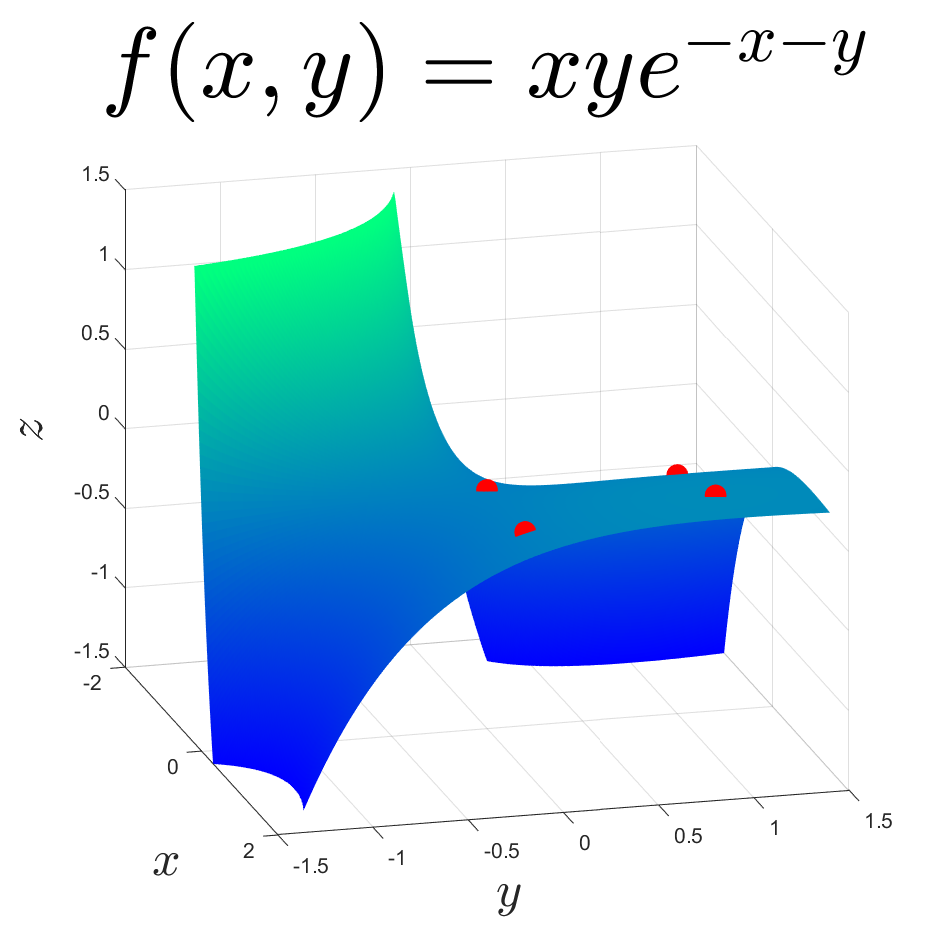
\includegraphics[width=0.6\textwidth]{./PS2_fig1.png}
	}
\end{center}

\pagebreak
\sol (c)\\
We expect \verb|fminsearch| to identify the one local maxima we identified, namely $(1,1)$ \\
\verb|PS2_script2.m| \hrule
\begin{lstlisting}{Matlab}
f = @(x,y) x.*y.*exp(-x-y);
negf = @(v) -f(v(1),v(2));
maxima = fminsearch(negf, [3, 3])
% Since we're looking for a maxima, we should negate the 
% function. This way, finding the minimum of negf, is 
% the same as finding the maximum of f.
% Also, since fminsearch expects to recieve a function 
% pointer, to a one-argument function, we have to
% make negf accept a vector as an argument, then extract
% the approriate x and y components.

fprintf('Local maxima found at (x, y) = (%.4f, %.4f)\n', ...
	maxima(1), maxima(2));
\end{lstlisting}
\verb|Output:|\\

\verb|Local maxima found at (x, y) = (1.0000, 1.0000)| \\

Which is what we expected. Therefore, we've demonstrated that we can use \verb|fminsearch| to identify local maxima on the function's surface.

\end{document}
